\section{Architecture}
\label{sec:architecture}

%  \begin{figure}[!htp]
%  \centering
% % 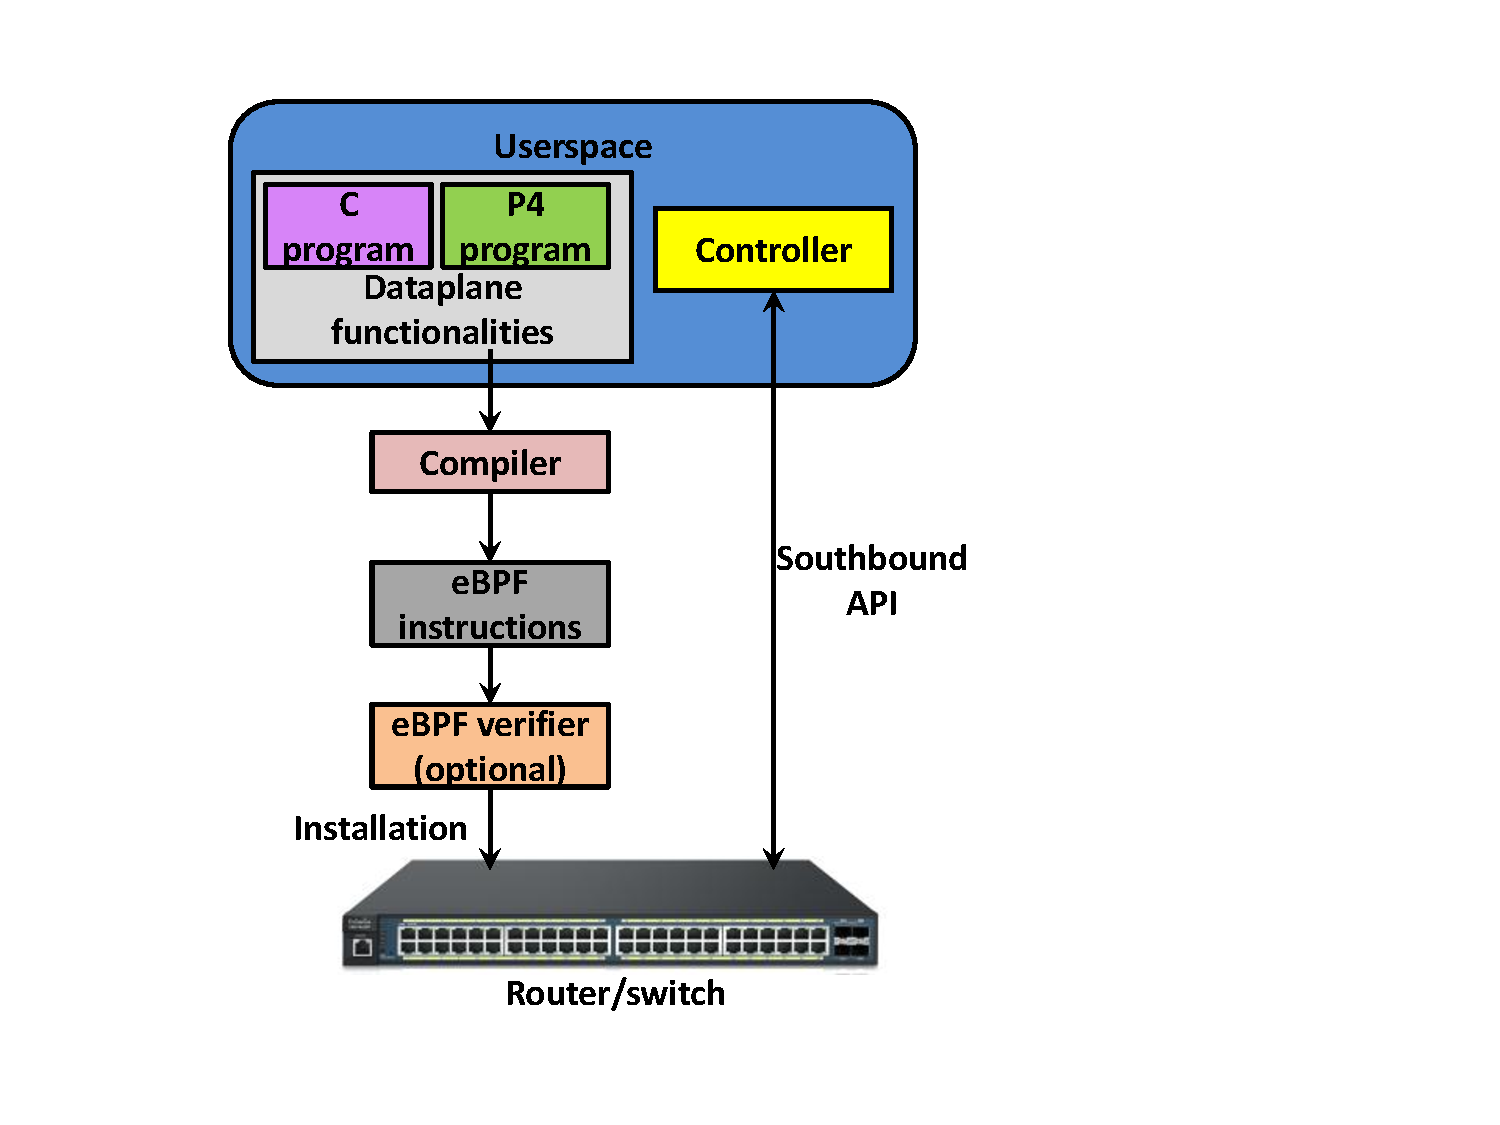
\includegraphics[width=.8\linewidth]{figures/Arquitetura2Crop.pdf}
% 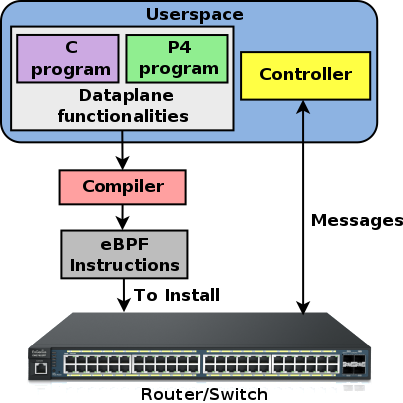
\includegraphics[width=.8\linewidth]{figures/03_fig01.png}
%  \caption{Architecture overview.}
%  \label{fig:03architecture}
%  \end{figure}

%Figure~\ref{fig:03architecture} provides an overview of the architecture.
The \system architecture has a logically centralized controller that communicates through a socket with the network elements (\eg routers, switches). 
Between the controller and the network elements, there is a southbound API that allows the controller to send platform-independent programs.

The controller can install programs in the data plane of the network elements at run time without network interruption (zero downtime), and it includes a scheduler to support multi-tenants and to move code in and out of the data plane.

% The advantage of this approach is that the parser, matching, and actions can be modified at runtime.


%\subsection{Dataplane}

% When designing the data plane, it should consider performance and how generic it is. It must be fast to be able to process the packets, presenting good network performance. Moreover,
% the set of instructions must be generic to allow the implementation of various functionalities.

Our system has a generic packet processor, with no pre-established behavior.
% The behavior of the device is defined by the set of instructions that accesses the packet headers, payload, and does the parser, matching, and actions at runtime.
eBPFlow contains a virtual engine to support reprogrammability on the fly.
The virtual engine follows the well-defined Instruction Set Architecture (ISA) of eBPF, which follows a RISC architecture and is already available in the Linux kernel and well-known in the Computer Networking community, providing compatibility with existing network projects.

% The system uses the eBPF packet processor.

\subsection{eBPF}

%cBPF
Berkeley Packet Filter (BPF)~\cite{McCanne:1993:BPF:1267303.1267305}, now referred as classic BPF (cBPF), is a ``virtual machine" (called ``pseudo-machine" originally) with a well-defined instruction set, which works as a low-level bytecode, conceptually similar to Java Virtual Machine (JVM) bytecode. It is mainly used for packet filtering by \textit{libpcap}, and is also present in \textit{tcpdump} and \textit{wireshark} tools.

%eBPF
eBPF (extended BFP) is an improvement of BPF in which the architecture has been expanded from 32 to 64 bits, increased the number of write registers from 2 to 10, and added support for table operations and function calls~\cite{eBPF}.
Whereas BPF has only forward jumps, eBPF can have jumps in both directions.
The Linux kernel, since version 3.18, allows userspace programs to install eBPF programs into the kernel. 
eBPF allows designing architectures independent of platforms or protocols.
No prior knowledge of the protocol or packet structure is required. 
The parsing starts when the system loads a packet into the eBPF data memory, and the execution of the eBPF instructions moves the packet fields into registers and makes the necessary comparisons.

\begin{comment}
\begin{figure*}[ht]
\centering
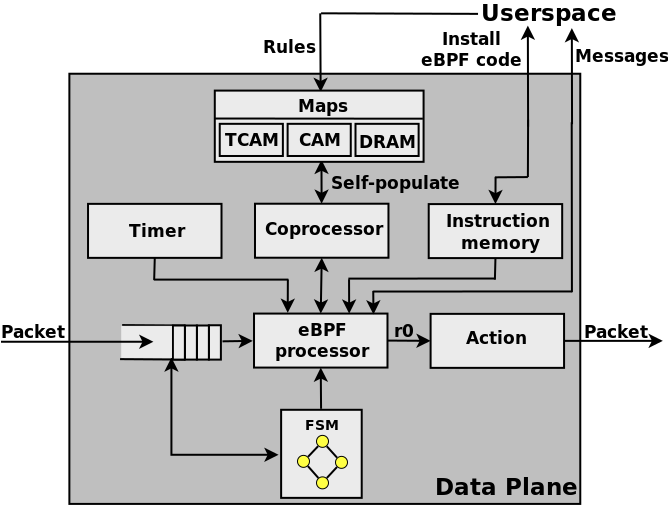
\includegraphics[width=.8\textwidth]{figures/06_fig01.png}
\caption{\system datapath implemented in NetFPGA SUME.}
\label{fig:06_fig01}
\end{figure*}
\end{comment}

%expressiveness
eBPF supports expressive flow rules.
%OpenFlow matching structure has some limitations.
It enables flow rules supporting inequality, complement (\texttt{not} operation), or range matching. 
For instance, it can do logical operations such as $\geq$ or $<$, which are needed for range expressions. 
By allowing the negation rule, packets that are not destined to port 80 (web traffic), for example, can be matched directly without the need to create rules for the other complement values, reducing the number of flow rules. 
% Moreover, OpenFlow switch can not extract Time-To-Live (TTL) or TCP Sequence Number fields, which are important to detect expiring packets and TCP migration, respectively. 
% The OpenFlow solution to extract fields that are not part of the OpenFlow standard is to do it at the OpenFlow controller. 
% On the other hand, an eBPF program containing only 6 instructions for each field can extract them.

%Top-of-Rack switches allows for approximately ~2000 OpenFlow flow entries.


%Table
The software implementation of eBPF in the Linux kernel supports a set of functions to handle maps ($< key; value >$ data structure). 
The most important functions are: \texttt{lookup}, \texttt{update}, and \texttt{delete}.The eBPF program can invoke these functions executing the eBPF call instruction.
The types of maps include arrays, hashmaps, hashmaps with Least Recently Used (LRU) replacement policy, and%, as of version 4.11,
longest-prefix match (LPM) using trie.
These maps allow eBPF programs to keep state between packet arrivals.
Classic Layer-2 switches use a hashmap to map the port associated to a MAC address.
LPM maps can be used to easily implement IP routing, mapping the port associated with a subnetwork.
Thus, maps are important to store states.
In our hardware implementation, our design choice is to use hardware modules. The maps are content-addressable memory (CAM) for exact-matching, ternary content-addressable memory (TCAM) for LPM, and Dynamic Random Access Memory (DRAM) for arrays.


\subsection{High-Level Languages}


High-level languages can be used to write code to the data plane and compile it into the eBPF instruction set. A subset of C already exists, which excludes some external libraries, system calls, and pointer arithmetic while providing functions for defining and manipulating tables. Since version 3.7, the LLVM compiler collection has a backend for the eBPF platform, allowing programming in this subset of C and generating executable code in eBPF format.

It is also possible to generate eBPF instructions through domain-specific languages, such as P4~\cite{Bosshart:2014:P4}.
There are efforts of the open source IOVisor project~\cite{IOvisor} and from VMware~\cite{p4c-xdp2018} that have already implemented a compiler from P4 to eBPF~\cite{P42EBPF2015}.
Thus, by choosing the eBPF instruction set, \system can also leverage previous C and P4 projects and applications.

% \begin{figure}[htb]
% \centering
% %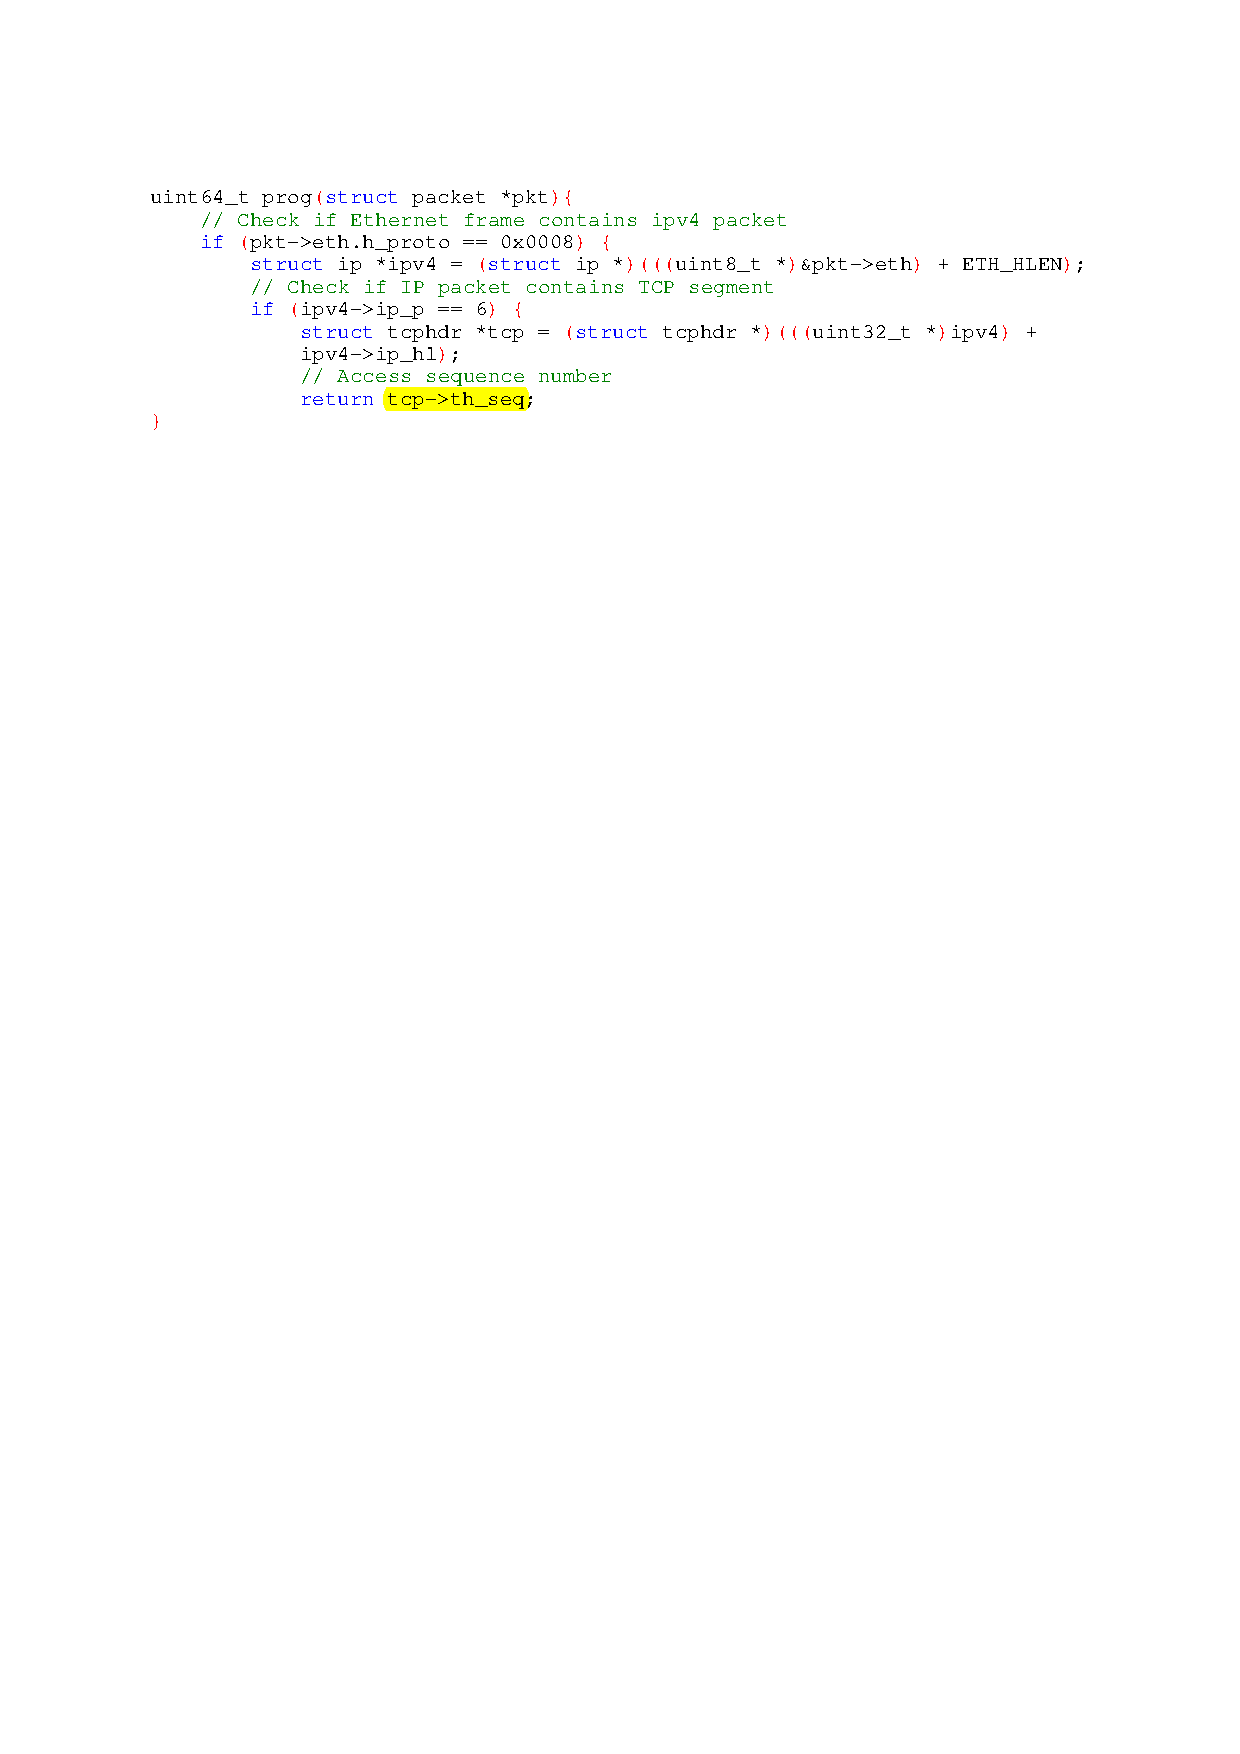
\includegraphics[width=1.\linewidth]{figures/sequenceNumber.pdf}
% 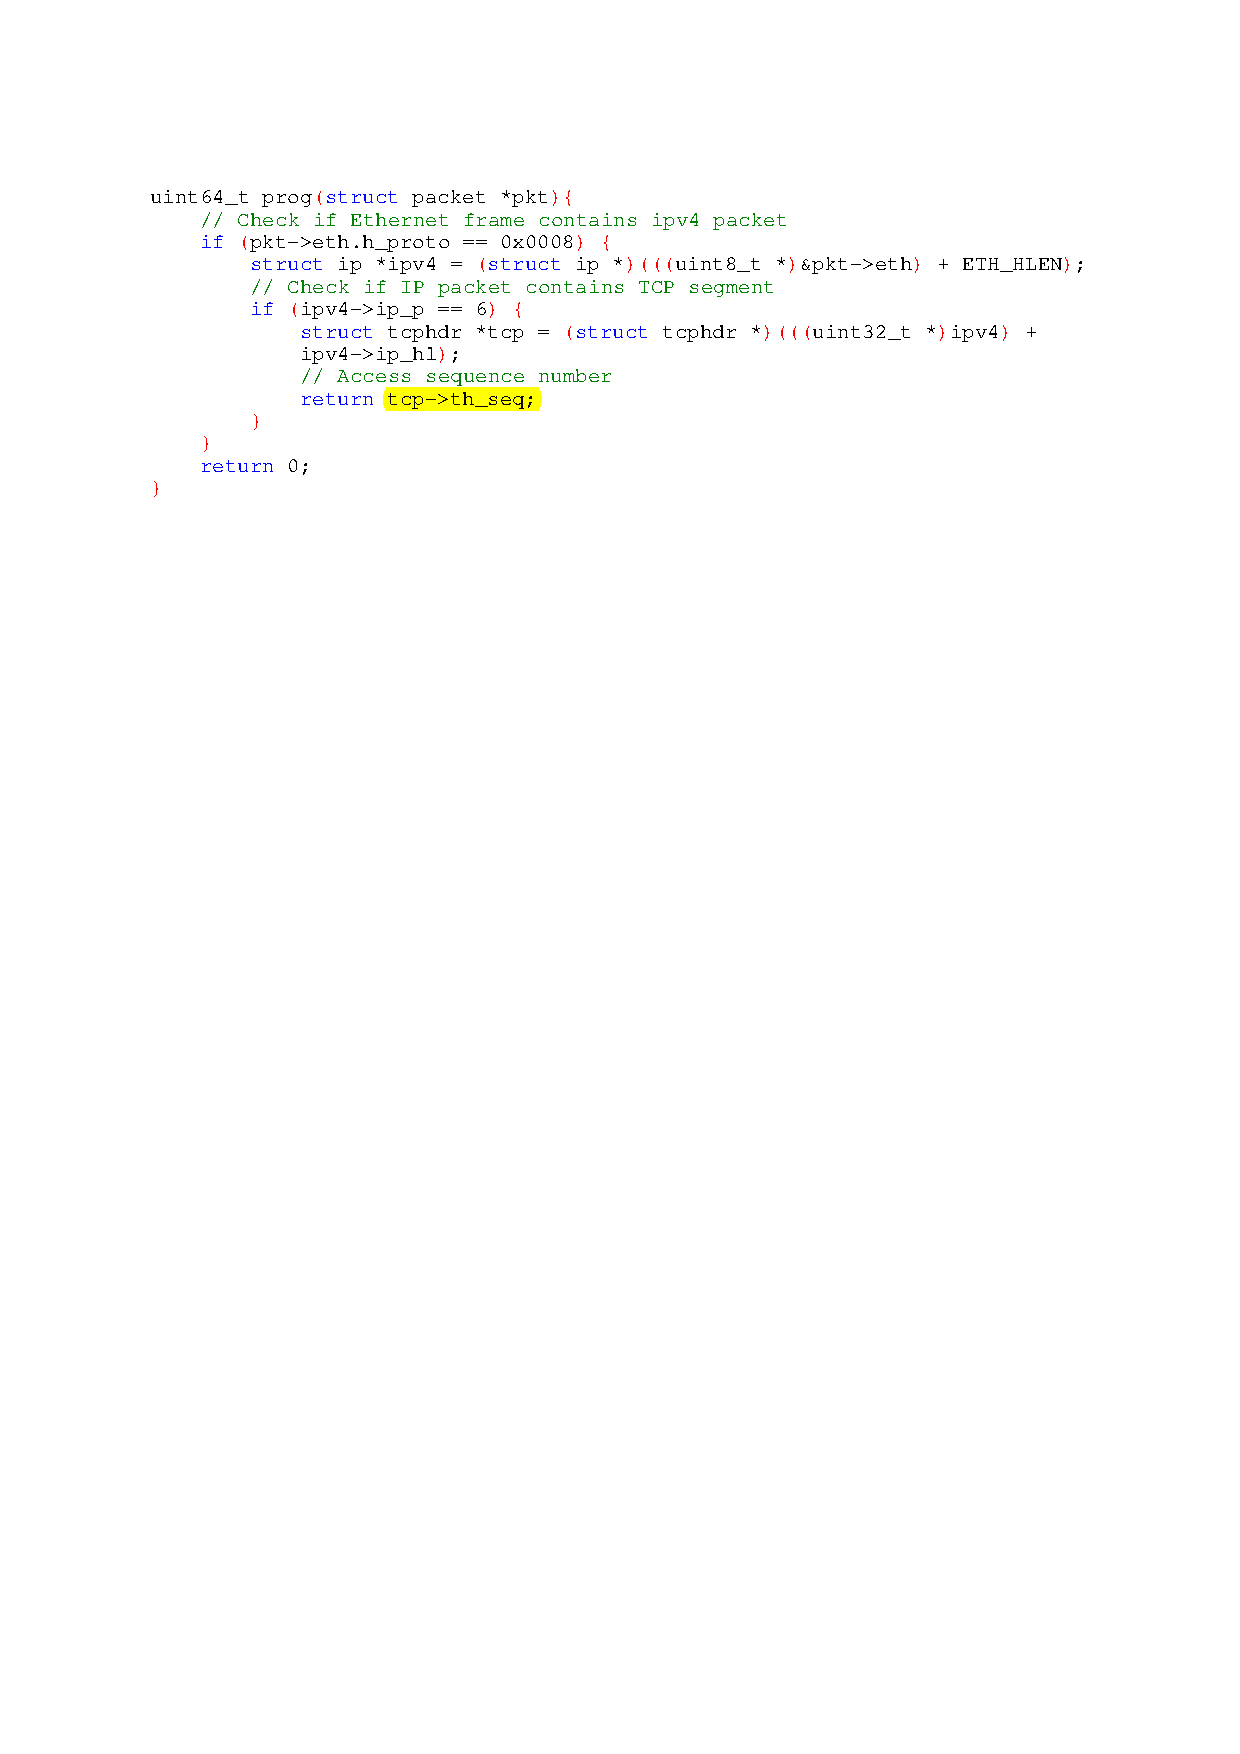
\includegraphics[width=1.\linewidth]{figures/seqnum.pdf}
% \caption{Example of a C program that accesses the TCP sequence number. This is not possible at the OpenFlow switch.}
% \label{fig:seqnum}
% \end{figure}

% Figure~\ref{fig:seqnum} illustrates an example of a field that can not be extracted at the OpenFlow switch but can be executed by eBPFlow: to analyze the TCP segment and access the sequence number.
% The code example, written in the subset of C, verifies that if it is an Ethernet frame that has an IP packet and contains a TCP segment. It then accesses the value of the TCP sequence number field. Dysco~\cite{Zave:2017:DSC:3098822.3098827} is an example of a system that provides a session protocol that requires the TCP sequence number.

% An important detail is that the LLVM compiler generates an executable in the executable and link format (ELF). This format has multiple segments for code execution. For our application, only the eBPF instruction set is required. The objdump tool allow to extract only the .text segment that has the instruction set. The controller installs this segment into the switch, which will execute these instructions.


% \begin{figure}[htb]
% \centering
% \includegraphics[width=.3\textwidth]{imagens/04_fig02.png}
% \caption{Diagrama de instalação das instruções eBPF no Switch/Roteador.}
% \label{fig:04_fig02}
% \end{figure}

%\subsection{Acyclic Control Flow Graph}
\subsection{eBPF verifier}
\label{sec:verifier}

%verifier
%There exits a verifier for programs with eBPF instructions.
The Linux kernel implementation provides an eBPF verifier.
The verifier checks the validity, security, and performance of eBPF programs.
If desired, the verifier allows eBPF programs with only bounded-loops to enable static analysis.
The eBPF verifier checks whether a program terminates, whether the memory accesses are in the range of memory space, and the greatest depth of the execution path (critical-path).
This critical-path can provide an upper-bound on the execution time.
The verifier aims to guarantee eBPF kernel-safe code execution.
In eBPFlow, the verifier can be used after the code has been compiled and before loading it into the data plane for static analysis.

The eBPF ISA is Turing complete but eBPF with Linux's verifier is not, because the verifier does not allow backward jumps.
In eBPFlow, we disable the backward jump in the verifier, thus, allowing our design to be Turing complete. We leave to the programmer the responsibility to check for infinite loops. The network manager writes a program in C or P4 language, and then compiles to eBPF. The eBPF program might be checked before installation with the eBPF verifier. The eBPF program is then installed on the device through a loading agent.


% \begin{figure}[htb]
% \centering
% %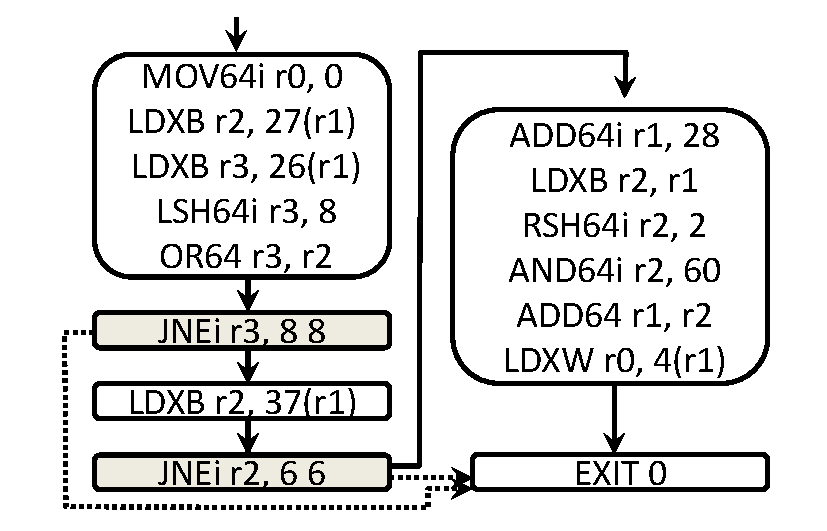
\includegraphics[width=.8\linewidth]{figures/eBPF_Acyclic_Control_Flow_Graph-_SeqNum3.pdf}
% 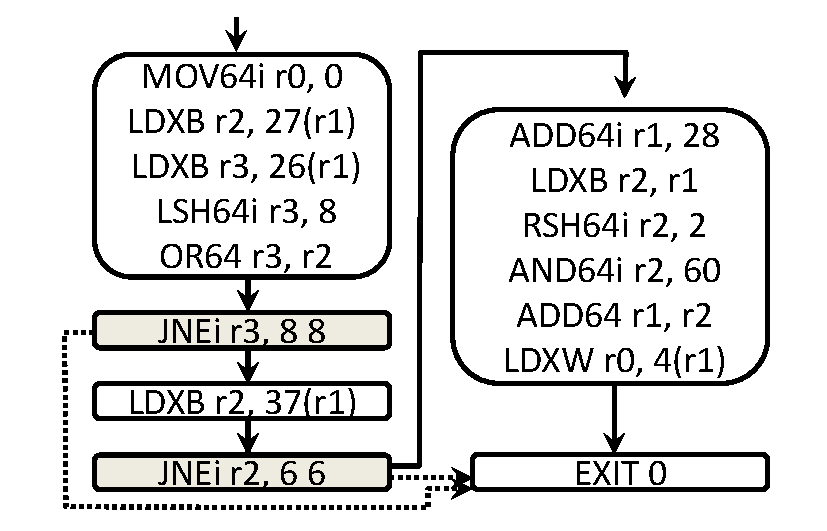
\includegraphics[width=.8\linewidth]{figures/eBPFACFG.pdf}
% \caption{eBPF Acyclic Control Flow Graph for the TCP sequence number example.}
% \label{fig:acfg}
% \end{figure}

% If the eBPF program has no backwards jump or just bound-loops (so loop unrolling can be applied), then the eBPF program can be synthesized into a directed Acyclic Control Flow Graph (ACFG). 
% Figure~\ref{fig:acfg} shows the ACFG to extract the TCP sequence number.% example presented in Figure~\ref{fig:seqnum}. 
% Each ACFG node contains one or more eBPF instructions. Instruction ending with the letter i indicates that the instruction uses an immediate value.

% The conditional jump nodes are the nodes that contain two output lines and light gray background.
% Solid line indicates the next ACFG node. Dotted line indicates a jump to another ACFG node.
% In our example, the conditional jump nodes contain the jump not equal (jnei) instruction.
% The last number of the jnei instruction indicates how many instructions to jump when the condition is valid.

% To better understand the eBPF program, let us explain that register r1 starts with a pointer to the packet and metadata (which we explain in Section~\ref{sec:metadata}) stored in the data memory and register r0 stores the return value.

% In the first node, load byte instructions extract the bytes 26 and 27 from the data memory.
% Given that the metadata has 16 bytes, this represents bytes 10 and 11 of the packet (counting from 0), which is the Ethernet type field. Then, a byte swap is done to set the endiness. 
% First jump instruction compares if the Ethernet type is 0x0800. Next, the IP protocol field is extracted from the IPv4 packet and checks if it is the TCP protocol (value 6). Finally, the TCP sequence number is extracted and placed in the return register (r0). The last instruction tells that the code terminates.
% ACFG is useful to determine the worst-case execution time.




%After presenting this example, we can better contextualize the general idea presented in  Figure~\ref{fig:03architecture}. In this scenario, 


%O roteador executa essas instruções para cada pacote recebido, permitindo um plano de dados com análise, casamento e ações dinâmicas.

% \subsection{Decoupling state from code}
% %\subsection{Self-Populate}
% \label{sec:selfpopulate}

% eBPF enables to decouple code and state.
% States are stored using maps.
% The code is used to parse the packet.
% For a matching, the code executes logical expressions and calls maps to query, for example, the next hop given the destination IP.
% For actions, the code can modify the packet and indicates to where the packet should be forwarded.

% Given this decoupling, the eBPFlow can self-populate the tables. The eBPF instruction can call the maps functions to insert, delete, or update the tables. This is not possible with current P4 or OpenFlow standard where
% the controller is responsible for making
% all the forwarding decision, resulting in additional 
% network traffic, latency, and controller overload.
% Moreover, if desired, the controller can query the content of the tables anytime, 
% %or be notified when a table entry is  modified, 
%  thus, still having the knowledge of the entire network.


\subsection{Southbound API}
\label{sec:southboundAPI}

\begin{table}[]
\caption{Messages exchanged between the controller and the network element.}
\begin{tabular}{|c|c|}
\hline
\textbf{Type of message} & \textbf{Description}                                                                        \\ \hline
Hi                       & Establish communication                                                                     \\ \hline
Allocate                 & \begin{tabular}[c]{@{}c@{}}Allocate eBPF program for certain \\ period of time\end{tabular} \\ \hline
\end{tabular}
\label{tbl:messages}
\end{table}
The controller and device communicate via socket through an agent running close to the device. After establishing the communication, both controller and agent can exchange messages with specific information. Table~\ref{tbl:messages} displays the supported messages between the controller and the network element.

Once the communication is established, the first message exchanged is the "Hi" message. 
It is sent to verify that the controller is connected to the network element and to obtain its identification number. 
The "Allocate" message contains the eBPF instructions that will be installed in the instruction memory of the eBPF processor and run for the duration specified on the message. The agent interacts with a local scheduler that is responsible for enforcing the requested duration and loading other allocation requests following a First Come First Serve (FCFS) policy and the duration for each request.

%\subsection{\red{Challenges}}

%\red{We present some challenges on implementation eBPFlow's design about NetFPGA.}  

%\begin{itemize}
%     %\item Double buffer system: ;  % not a challenge, it's a solution
%     %\item Packet zero copy: ;   % not a challenge, it's a solution
%     \item Restrictions of time: ;  
%\end{itemize}
